%!TeX program = xelatex
\documentclass[12pt,hyperref,a4paper,UTF8]{ctexart}
\usepackage{ZJUTReport}
\usepackage{listings}
\usepackage{xcolor}
\usepackage{tikz}
\usepackage{array}
\usepackage{booktabs}
\usepackage{placeins}
\usepackage{tabularx}
\usetikzlibrary{positioning,arrows.meta}

\usepackage{setspace}
\setstretch{1.5} % 设置全局行距为1.5倍
\hyphenpenalty=10000\relax
\exhyphenpenalty=10000\relax
\emergencystretch=3em\relax
\usepackage{etoolbox}
\newcolumntype{L}[1]{>{\centering\arraybackslash}p{#1}}
\newcolumntype{Y}{>{\centering\arraybackslash}X}
\newcolumntype{C}[1]{>{\centering\arraybackslash}p{#1}}
\AtBeginEnvironment{table}{%
    \setstretch{1.0}%
    \setlength{\tabcolsep}{3.5pt}%
    \renewcommand{\arraystretch}{1.10}%
}
\AtBeginEnvironment{tabularx}{\fontsize{9pt}{10.8pt}\selectfont}
\captionsetup[table]{font=footnotesize,skip=4pt}

\usepackage{enumitem} % 载入enumitem包以便自定义列表环境
\setlist[itemize]{itemsep=0pt, parsep=0pt} % 设置itemize环境的项目间距和段落间距

\setmainfont{Times New Roman} % 英文正文为Times New Roman

%封面页设置
{   
    %标题
    \title{ 
        \vspace{1cm}
        \heiti \Huge {Java应用课程设计报告} \par
        \vspace{1cm} 
        \heiti \Large {\underline{基于MQTT协议的企业设备}} \\
        \heiti \Large {\underline{运行监测与远程控制系统}}
        \vspace{1cm}
    }

    \author{
        \vspace{0.5cm}
        \kaishu\Large 姓\qquad 名\ \dlmu[9cm]{XXX} \\ %姓名
        \vspace{0.5cm}
        \kaishu\Large 学\qquad 号\ \dlmu[9cm]{2023XXXXXX} \\ %学号
        \vspace{0.5cm}
        \kaishu\Large 指导老师\ \dlmu[9cm]{XXX} \\ %指导老师
        \vspace{0.5cm}
        \kaishu\Large 专业班级\ \dlmu[9cm]{智能科学与技术} \\ %专业班级
        \vspace{0.5cm}
        \kaishu\Large 学\qquad 院\ \dlmu[9cm]{信息工程学院} \\ %学院
    }
        
    \date{\today} % 默认为今天的日期，可以注释掉不显示日期
}
%%------------------------document环境开始------------------------%%
\begin{document}

%%-----------------------封面--------------------%%
\cover
\thispagestyle{empty} % 封面不显示页码

%%--------------------------目录页------------------------%%
\pagenumbering{Roman} % 前置部分使用罗马数字页码
\newpage
\begingroup
\small
\setstretch{1.0}
\tableofcontents
\endgroup

%%------------------------正文页从这里开始-------------------%%
\newpage
\pagenumbering{arabic} % 正文使用阿拉伯数字页码
\setcounter{page}{1} % 页码从 1 开始

%%==================== 1 课程设计任务书 ====================%%
\section{课程设计任务书}

\subsection{设计任务与目标}

本课程设计的设计任务是：设计并实现一个面向企业的设备运行监测与远程控制系统。系统以 MQTT 协议作为设备与服务器之间的通信协议，以 B/S（浏览器/服务器）架构向用户提供统一的操作界面，实现多台设备的集中监测与远程控制。具体设计目标如下：

\begin{enumerate}
    \item 实现设备台账管理，能够对设备、设备属性（采集点 AI）与控制参数（控制点 DO）进行新增、删除、修改、查询；
    \item 通过 MQTT 协议订阅采集主题 \texttt{/kettle/pub}，自动接收设备上报的运行数据，解析 JSON 数据帧并写入数据库；
    \item 实现远程控制，向主题 \texttt{/\{devId\}/sub} 下发按规范封装的 JSON 控制帧；
    \item 提供基本信息统计报表与图形化分析报表；
    \item 实现基于角色的权限管理（RBAC），保证不同角色只能访问被授权的功能；
    \item 系统界面规范、操作符合用户习惯，程序运行稳定无错误。
\end{enumerate}

\subsection{选题背景介绍}

随着工业企业设备数量不断增加，传统的人工巡检与纸质记录方式已难以满足设备运行状态的实时监测与集中管控需求。一方面，设备数据分散、采集不及时，故障难以及时发现；另一方面，设备控制依赖现场人工操作，运维成本高、响应速度慢。因此，构建一套能够自动采集设备运行数据、支持远程控制、并提供可视化统计分析的信息化系统具有重要的现实意义。

在通信技术上，MQTT（Message Queuing Telemetry Transport）是一种基于发布/订阅模式的轻量级物联网通信协议，具有开销小、支持低带宽网络、一对多消息分发等特点，广泛应用于物联网与工业设备互联场景。在系统架构上，B/S 架构无需在客户端安装专用软件，便于部署与维护，符合企业级应用的使用习惯。

综上，本设计选择「MQTT + B/S」的技术路线，构建一套企业设备运行监测与远程控制系统，实现设备数据的自动汇聚、可视化分析与远程控制，助力企业降本增效。

%%==================== 2 方案设计与功能说明 ====================%%
\section{方案设计与功能说明}

\subsection{总体方案设计}

系统采用分层架构设计，自上而下分为表示层、业务层、数据层，并辅以独立的 MQTT 通信层，整体架构如\autoref{fig:arch}所示。

\begin{figure}[!htbp]
    \centering
    \begin{tikzpicture}[
        node distance=0.85cm,
        box/.style={rectangle,draw,rounded corners,align=center,minimum width=8.2cm,minimum height=0.95cm,font=\small},
        arrow/.style={-{Stealth},thick}]
        \node[box,fill=blue!8] (a) {表示层：Vue3 + Element Plus + ECharts（浏览器）};
        \node[box,fill=orange!10,below=of a] (b) {业务层：Spring Boot（Controller $\rightarrow$ Service $\rightarrow$ Repository）\\ 内含 安全模块（JWT+RBAC） 与 MQTT 客户端（Paho）};
        \node[box,fill=green!10,below=of b] (c) {数据层：MySQL 数据库};
        \node[box,fill=gray!10,below=of c] (d) {MQTT Broker（Moquette，内嵌）};
        \node[box,fill=gray!10,below=of d] (e) {设备采集器 / 数据模拟器};
        \draw[arrow] (a) -- node[right,font=\small]{HTTP / HTTPS（JWT）} (b);
        \draw[arrow] (b) -- node[right,font=\small]{JDBC} (c);
        \draw[arrow] (b.west) to[out=-140,in=140] node[left,font=\small]{MQTT} (d.west);
        \draw[arrow] (d) -- node[right,font=\small]{MQTT 发布/订阅} (e);
    \end{tikzpicture}
    \caption{系统总体架构}
    \label{fig:arch}
\end{figure}

各层职责如下：

\begin{itemize}
    \item \textbf{表示层}：基于 Vue 3 + Element Plus 组件库 + ECharts 图表库，负责界面展示与用户交互，通过 HTTP 接口与后端通信，并携带 JWT 令牌完成身份认证；
    \item \textbf{业务层}：基于 Spring Boot 框架，采用 Controller $\rightarrow$ Service $\rightarrow$ Repository 的分层结构，实现业务逻辑、权限校验、数据校验与事务管理；其中安全模块负责登录认证与权限控制，MQTT 客户端模块负责订阅采集消息与发布控制消息；
    \item \textbf{数据层}：采用 MySQL 数据库与 Spring Data JPA 持久化框架，存储用户、角色、权限、设备、点位、采集数据与控制记录等业务数据；
    \item \textbf{MQTT 通信层}：后端作为 MQTT 客户端订阅采集主题、发布控制主题，与设备采集器之间通过 MQTT Broker 进行消息收发。
\end{itemize}

系统主要技术选型如\autoref{tab:tech}所示，其中后端采用 Spring Boot 与 Spring Security，前端采用 Vue，数据库采用 MySQL，身份认证采用 JWT，MQTT 通信采用 Eclipse Paho 与 Moquette Broker。

\begin{table}[!htbp]
    \centering
    \caption{系统技术选型}
    \label{tab:tech}
    \begin{tabularx}{0.90\textwidth}{@{}L{2.2cm} L{5.3cm} Y@{}}
    \toprule
    \textbf{层次} & \textbf{技术} & \textbf{说明} \\
    \midrule
    后端框架 & Spring Boot 3.3、Java 21 & 分层开发、依赖注入、自动配置 \\
    数据访问 & Spring Data JPA & 实体映射与 CRUD \\
    数据库 & MySQL 8/9 & 关系型数据库 \\
    安全 & Spring Security + JWT & 认证与 RBAC 授权 \\
    消息通信 & Eclipse Paho + Moquette & MQTT 客户端与内嵌 Broker \\
    前端 & Vue 3 + Vite + Element Plus + ECharts & SPA 单页应用 \\
    \bottomrule
    \end{tabularx}
\end{table}

\subsection{功能模块设计}

系统在功能上划分为登录认证与权限、设备管理、MQTT 数据采集、远程控制、数据查询与图形分析、统计报表六大模块，各模块设计如下。

\subsubsection{登录认证与权限模块}

登录认证与权限模块负责用户登录、退出和当前用户信息获取，以及用户、角色、菜单权限的增删改查，并根据 RBAC 权限动态渲染前端菜单与按钮。系统基于 Spring Security 采用 JWT 无状态认证：登录成功后校验用户名与 BCrypt 加密密码，签发有效期为 24 小时的 JWT 令牌并返回角色编码、权限标识与菜单树；后续请求由 \texttt{JwtAuthenticationFilter} 解析令牌、重建安全上下文，再通过 \texttt{@PreAuthorize} 完成接口授权。对外接口包括登录 \texttt{POST /api/auth/login}、当前用户 \texttt{GET /api/auth/me}、退出 \texttt{POST /api/auth/logout}，用户、角色与权限的 CRUD 接口，以及角色授权 \texttt{PUT /api/roles/\{id\}/permissions}。远程控制操作同时记录操作人与时间，形成审计日志。

\subsubsection{设备管理模块}

设备管理模块维护设备编号、名称、类型、型号、厂商、位置、状态和安装日期等台账信息，以及量程、单位、缺省值等设备点位属性。点位分为采集点（AI，类型 1）与控制点（DO，类型 2），与设备构成一对多关系；业务流程按照搜索、分页展示和新增、编辑、删除展开，删除设备时级联清理关联点位以保证数据一致性。设备分页、详情及增删改接口分别为 \texttt{GET /api/devices}、\texttt{GET /api/devices/\{id\}} 和 \path{POST/PUT/DELETE /api/devices}，点位分页及增删改接口为 \texttt{GET /api/points} 和 \path{POST/PUT/DELETE /api/points}。

\subsubsection{MQTT 数据采集模块}

MQTT 数据采集模块在后端启动时创建客户端并订阅主题 \texttt{/kettle/pub}，接收设备运行数据、解析 JSON 数据帧、写入数据库并更新设备在线状态，连接中断后自动重连。消息到达后，系统提取 \texttt{devId}、\texttt{msgType} 与 \texttt{data} 字段；当消息类型为 \texttt{aiValueRpt} 时遍历各点位值并写入采集数据表。该模块通过 MQTT 回调与内部服务完成处理，不直接提供 HTTP 接口，其结果由数据查询模块对外展示，具体流程见\autoref{fig:flow}（左图）。

\subsubsection{远程控制模块}

远程控制模块允许用户选择设备与控制点并设置目标值。系统先校验 \texttt{control:send} 权限，再封装消息类型为 \texttt{doValueRpt} 的 JSON 控制帧，发布到主题 \texttt{/\{devId\}/sub}，同时将状态为“已发送”的记录写入控制记录表以供审计追溯。设备执行回执的解析和记录状态更新属于预留扩展机制，不在本期实现范围内；控制下发与记录查询接口分别为 \texttt{POST /api/control/send} 和 \texttt{GET /api/control/records}，具体流程见\autoref{fig:flow}（右图）。

\begin{figure}[!htbp]
    \centering
    \begin{minipage}[t]{0.47\textwidth}
        \centering
        \begin{tikzpicture}[
            node distance=0.7cm,
            startstop/.style={rectangle,rounded corners,draw,minimum width=5.9cm,minimum height=0.85cm,align=center,font=\small},
            arrow/.style={-{Stealth},thick}]
            \node[startstop,fill=gray!10] (s1) {采集器发布 \texttt{aiValueRpt} 数据帧};
            \node[startstop,below=of s1] (s2) {MQTT Broker 主题 \texttt{/kettle/pub}};
            \node[startstop,below=of s2] (s3) {后端 MQTT 订阅回调};
            \node[startstop,below=of s3] (s4) {校验 \texttt{devId}、\texttt{msgType} 并解析 JSON};
            \node[startstop,below=of s4] (s5) {遍历 \texttt{data} 中各点位};
            \node[startstop,below=of s5] (s6) {批量写入 \texttt{device\_data} 并更新在线状态};
            \draw[arrow] (s1)--(s2);
            \draw[arrow] (s2)--(s3);
            \draw[arrow] (s3)--(s4);
            \draw[arrow] (s4)--(s5);
            \draw[arrow] (s5)--(s6);
        \end{tikzpicture}\\
        {\small（a）数据采集处理流程}
    \end{minipage}
    \hfill
    \begin{minipage}[t]{0.47\textwidth}
        \centering
        \begin{tikzpicture}[
            node distance=0.7cm,
            startstop/.style={rectangle,rounded corners,draw,minimum width=5.9cm,minimum height=0.85cm,align=center,font=\small},
            arrow/.style={-{Stealth},thick}]
            \node[startstop,fill=gray!10] (c1) {用户在界面选择设备与控制点、填写目标值};
            \node[startstop,below=of c1] (c2) {后端校验权限（\texttt{control:send}）};
            \node[startstop,below=of c2] (c3) {封装 \texttt{doValueRpt} JSON 控制帧};
            \node[startstop,below=of c3] (c4) {MQTT 发布到主题 \texttt{/\{devId\}/sub}};
            \node[startstop,below=of c4] (c5) {写入 \texttt{control\_record} 控制记录};
            \node[startstop,below=of c5] (c6) {设备接收控制帧并执行};
            \draw[arrow] (c1)--(c2);
            \draw[arrow] (c2)--(c3);
            \draw[arrow] (c3)--(c4);
            \draw[arrow] (c4)--(c5);
            \draw[arrow] (c5)--(c6);
        \end{tikzpicture}\\
        {\small（b）远程控制处理流程}
    \end{minipage}
    \caption{MQTT 数据采集与远程控制处理流程}
    \label{fig:flow}
\end{figure}

\subsubsection{数据查询与图形分析模块}

数据查询与图形分析模块支持按设备、点位和时间范围分页查询历史采集数据，提供各点位最新值看板，并通过折线图展示运行趋势及最大值、最小值、平均值。查询服务基于 JPA Specification 动态拼接条件，按采集时间倒序分页返回；图形分析则按时间升序组装时间序列与数值序列，交由 ECharts 渲染。数据分页、最新值和趋势图接口依次为 \texttt{GET /api/data}、\texttt{GET /api/data/latest} 和 \texttt{GET /api/data/chart}。

\subsubsection{统计报表模块}

统计报表模块汇总设备总量、在线数、点位总数、今日数据量和控制次数，展示设备类型分布，并对指定点位进行数值统计。汇总数据由各实体仓库的计数方法聚合得到，设备类型分布通过分组统计生成，趋势和点位统计复用数据查询模块。对应接口为汇总 \texttt{GET /api/dashboard/summary}、类型分布 \texttt{GET /api/dashboard/deviceTypeDist}、趋势 \texttt{GET /api/dashboard/dataTrend} 和点位统计 \texttt{GET /api/dashboard/pointStats}。

\subsection{通信报文与接口示例}

\subsubsection{MQTT 数据帧格式}

设备上报的采集数据帧（主题 \texttt{/kettle/pub}，消息类型 \texttt{aiValueRpt}）格式如下：

\begin{verbatim}
{
    "devId":"492C230518046576",
    "msgType":"aiValueRpt",
    "data":{"AI1":"0","AI2":"4889","AI3":"0","AI4":"20"},
    "timestamp":"1688344552"
}
\end{verbatim}

系统下发的控制数据帧（主题 \texttt{/\{devId\}/sub}，消息类型 \texttt{doValueRpt}）格式如下：

\begin{verbatim}
{
    "devId":"492C230518046576",
    "msgType":"doValueRpt",
    "data":{"DO1":"0","DO2":"0","DO3":"0","DO4":"0"},
    "timestamp":"1687333310"
}
\end{verbatim}

数据帧各字段含义如\autoref{tab:frame}所示。

\begin{table}[!htbp]
    \centering
    \caption{MQTT 数据帧字段含义}
    \label{tab:frame}
    \begin{tabularx}{0.90\textwidth}{@{}L{2.2cm} L{2.0cm} Y@{}}
    \toprule
    \textbf{字段} & \textbf{类型} & \textbf{说明} \\
    \midrule
    devId & String & 设备唯一标识，用于定位设备 \\
    msgType & String & 消息类型：aiValueRpt 采集上报、doValueRpt 控制下发 \\
    data & Object & 点位键值对，键为点位编码（AI1$\sim$AI4、DO1$\sim$DO4） \\
    timestamp & String & Unix 时间戳（秒） \\
    \bottomrule
    \end{tabularx}
\end{table}

\subsubsection{核心接口请求与响应示例}

\textbf{登录接口} \texttt{POST /api/auth/login} 的请求体与实际响应如下：

\begin{verbatim}
请求：{"username":"admin","password":"123456"}
响应：{"code":200,"message":"success",
      "data":{"token":"<JWT>","user":{...}}}
\end{verbatim}

\textbf{汇总统计接口} \texttt{GET /api/dashboard/summary} 的实际响应如下：

\begin{verbatim}
{"code":200,"message":"success","data":
 {"deviceTotal":3,"deviceOnline":3,"pointTotal":16,
  "dataToday":19572,"controlTotal":3}}
\end{verbatim}

\textbf{数据分页查询接口} \texttt{GET /api/data} 的响应 \texttt{data} 中，\texttt{records} 为记录数组，\texttt{total} 为总条数。

\textbf{控制下发接口} \texttt{POST /api/control/send} 的请求体与实际响应如下：

\begin{verbatim}
请求：{"devId":"492C230518046576","data":{"DO1":"1"}}
响应：{"code":200,"message":"success","data":
 {"topic":"/492C230518046576/sub","sent":true,
  "records":[{"pointCode":"DO1","value":"1","status":true}]}}
\end{verbatim}

%%==================== 3 程序框图 ====================%%
\section{程序框图}

\subsection{系统总体架构图}

系统总体架构见\autoref{fig:arch}。后端采用分层架构，自顶向下依次为 Controller（控制层）、Service（业务层）、Repository（数据访问层），并辅以 Security（安全）与 MQTT 两个横切模块。

\subsection{后端分层与类间关系}

\begingroup
\small
后端各层之间通过依赖注入建立调用关系。\textbf{控制层（Controller）}包括 AuthController、UserController、RoleController、PermissionController、DeviceController、DevicePointController、DataController、ControlController 和 DashboardController，负责接收 HTTP 请求、校验参数并调用业务层；\textbf{业务层（Service）}包括 AuthService、UserService、RoleService、PermissionService、DeviceService、DevicePointService、DataService、ControlService 和 DashboardService，负责业务逻辑与事务管理；\textbf{数据访问层（Repository）}包括 UserRepository、RoleRepository、PermissionRepository、DeviceRepository、DevicePointRepository、DeviceDataRepository 和 ControlRecordRepository，负责数据持久化操作。

安全模块由 SecurityConfig、JwtAuthenticationFilter、JwtUtil 和 SecurityUtils 组成，负责登录认证与权限校验；MQTT 模块由 MqttService、DataCollectionService、EmbeddedBroker 和 DeviceSimulator 组成，负责消息收发、数据解析与模拟上报。

各层之间的调用关系为：Controller 调用 Service，Service 调用 Repository；MQTT 消息回调 MqttService 后转入 DataCollectionService 完成数据入库；权限过滤发生在请求进入 Controller 之前。后端核心类图如\autoref{fig:class}所示（图中仅列出代表性类，其余类结构类似）。
\endgroup

\begin{figure}[!htbp]
    \centering
    \begin{tikzpicture}[
        node distance=0.8cm and 1.1cm,
        cls/.style={rectangle,draw,align=left,font=\small,minimum width=3.5cm,minimum height=1.15cm},
        iface/.style={rectangle,draw,dashed,align=left,font=\small,minimum width=3.5cm,minimum height=0.9cm},
        arrow/.style={-{Stealth},thick}]
        \node[cls,fill=blue!6] (authc) {\textbf{AuthController}\\ login(\dots)、me()};
        \node[cls,fill=blue!6,right=of authc] (datac) {\textbf{DataController}\\ page(\dots)、chart(\dots)};
        \node[cls,fill=blue!6,right=of datac] (ctrl) {\textbf{ControlController}\\ send(\dots)、records()};
        \node[cls,fill=orange!8,below=of authc] (auths) {\textbf{AuthService}\\ login(\dots)\\ buildUserInfo()};
        \node[cls,fill=orange!8,below=of datac] (datas) {\textbf{DataService}\\ page(\dots)、chart(\dots)};
        \node[cls,fill=orange!8,below=of ctrl] (ctrls) {\textbf{ControlService}\\ send(\dots)、records()};
        \node[iface,below=of auths] (userr) {\textbf{UserRepository}\\ findByUsername()};
        \node[iface,below=of datas] (datar) {\textbf{DeviceDataRepository}\\ stats(\dots)};
        \node[iface,below=of ctrls] (recr) {\textbf{ControlRecordRepository}};
        \node[cls,fill=green!8,below=1.2cm of datar] (mqtt) {\textbf{MqttService}\\ publish(\dots)\\ messageArrived()};
        \node[cls,fill=green!8,right=of mqtt] (coll) {\textbf{DataCollectionService}\\ handle(\dots)\\ handleAiReport()};
        \draw[arrow] (authc) -- (auths);
        \draw[arrow] (datac) -- (datas);
        \draw[arrow] (ctrl) -- (ctrls);
        \draw[arrow] (auths) -- (userr);
        \draw[arrow] (datas) -- (datar);
        \draw[arrow] (ctrls) -- (recr);
        \draw[arrow] (mqtt) -- (coll);
        \draw[arrow] (coll) -- node[right,font=\small]{入库} (datar);
    \end{tikzpicture}
    \caption{后端核心类图（分层与调用关系）}
    \label{fig:class}
\end{figure}

\subsection{核心算法原理}

系统的核心算法覆盖身份认证、数据帧解析与菜单树构建。用户登录成功后，服务端以密钥对用户标识和过期时间进行 HMAC 签名，生成 JWT 令牌；客户端后续携带令牌，服务端校验签名与有效期后重建身份和权限。对于订阅到的 JSON 数据帧，系统先按 \texttt{devId} 定位设备，再按 \texttt{msgType} 分发处理；当类型为 \texttt{aiValueRpt} 时，遍历 \texttt{data} 中的键值对，将字符串数值转换后批量写入数据库。菜单树则根据用户拥有的目录与菜单权限，按照父子关系自顶向下组装，供前端动态渲染侧边菜单。

%%==================== 4 主要程序清单与数据结构设计 ====================%%
\section{主要程序清单与数据结构设计}

\subsection{主要程序清单}

本节按照课程设计要求，仅给出核心类的数据成员、方法名、返回值、参数及调用关系说明，不粘贴源代码。

\subsubsection{程序总体结构与调用关系}

系统程序的整体调用关系如下：浏览器通过 HTTP 请求访问 Controller 层接口；Controller 校验参数后调用对应 Service 层方法；Service 层处理业务逻辑并通过 Repository 层完成数据持久化；MQTT 消息由 MqttService 接收后转交 DataCollectionService 解析入库；登录认证由 JwtAuthenticationFilter 拦截请求并结合 JwtUtil 完成。

\subsubsection{核心服务类方法清单}

AuthService（登录认证服务）的方法清单如\autoref{tab:authservice}所示。

\begin{table}[!htbp]
    \centering
    \caption{AuthService 方法清单}
    \label{tab:authservice}
    \begin{tabularx}{0.90\textwidth}{@{}L{3.2cm} L{3.4cm} L{2.3cm} Y@{}}
    \toprule
    \textbf{方法} & \textbf{参数} & \textbf{返回值} & \textbf{说明} \\
    \midrule
    login & username, password & Map & 校验账号密码与状态，生成 JWT 并返回令牌与用户信息 \\
    currentUser & — & UserInfoVO & 返回当前登录用户及其角色、权限、菜单 \\
    buildUserInfo & User & UserInfoVO & 汇总角色编码、权限标识与菜单树 \\
    \bottomrule
    \end{tabularx}
\end{table}

JwtUtil（令牌工具类）与 SecurityUtils（安全上下文工具类）的方法清单如\autoref{tab:jwtutil}所示。

\begin{table}[!htbp]
    \centering
    \caption{JwtUtil 与 SecurityUtils 方法清单}
    \label{tab:jwtutil}
    \begin{tabularx}{0.90\textwidth}{@{}L{3.2cm} L{3.4cm} L{2.3cm} Y@{}}
    \toprule
    \textbf{方法} & \textbf{参数} & \textbf{返回值} & \textbf{说明} \\
    \midrule
    generateToken & userId, username & String & 生成带过期时间的 JWT 令牌 \\
    parse & token & Claims & 解析并校验令牌，返回载荷 \\
    getUsername & token & String & 从令牌中获取用户名 \\
    validate & token & boolean & 判断令牌是否有效 \\
    getCurrentUser & — & User & 从安全上下文获取当前用户 \\
    \bottomrule
    \end{tabularx}
\end{table}

UserService（用户管理服务）的方法清单如\autoref{tab:userservice}所示。

\begin{table}[!htbp]
    \centering
    \caption{UserService 方法清单}
    \label{tab:userservice}
    \begin{tabularx}{0.90\textwidth}{@{}L{3.2cm} L{3.4cm} L{2.3cm} Y@{}}
    \toprule
    \textbf{方法} & \textbf{参数} & \textbf{返回值} & \textbf{说明} \\
    \midrule
    page & keyword, page, size & PageResult & 按关键字分页查询用户 \\
    create & UserSaveDTO & void & 新增用户并分配角色 \\
    update & id, UserSaveDTO & void & 修改用户信息与角色 \\
    delete & id & void & 删除用户 \\
    updateStatus & id, status & void & 启用/停用用户 \\
    resetPassword & id, password & void & 重置用户密码 \\
    \bottomrule
    \end{tabularx}
\end{table}

DeviceService（设备管理服务）与 DevicePointService（点位管理服务）的方法清单如\autoref{tab:deviceservice}所示。

\begin{table}[!htbp]
    \centering
    \caption{DeviceService / DevicePointService 方法清单}
    \label{tab:deviceservice}
    \begin{tabularx}{0.90\textwidth}{@{}L{3.2cm} L{3.4cm} L{2.3cm} Y@{}}
    \toprule
    \textbf{方法} & \textbf{参数} & \textbf{返回值} & \textbf{说明} \\
    \midrule
    page & keyword, status, type, page, size & PageResult & 按条件分页查询设备 \\
    create & Device & void & 新增设备（校验编号唯一） \\
    update & id, Device & void & 修改设备信息 \\
    delete & id & void & 删除设备并级联删除点位 \\
    listByDevice & deviceId & List & 查询某设备的全部点位 \\
    create(点) & DevicePoint & void & 新增点位（校验编码唯一） \\
    \bottomrule
    \end{tabularx}
\end{table}

DataService（数据服务）与 ControlService（控制服务）的方法清单如\autoref{tab:dataservice}所示。

\begin{table}[!htbp]
    \centering
    \caption{DataService / ControlService 方法清单}
    \label{tab:dataservice}
    \begin{tabularx}{0.90\textwidth}{@{}L{3.2cm} L{3.4cm} L{2.3cm} Y@{}}
    \toprule
    \textbf{方法} & \textbf{参数} & \textbf{返回值} & \textbf{说明} \\
    \midrule
    page & devId, pointCode, start, end, page, size & PageResult & 按条件分页查询采集数据 \\
    latest & devId & List & 查询设备各采集点最新值 \\
    chart & devId, pointCode, start, end & Map & 组装时间/数值序列供绘图 \\
    pointStats & devId, pointCode, start, end & Map & 统计点位最大/最小/平均值 \\
    send & devId, data & Map & 封装控制帧、发布并记录 \\
    records & devId, page, size & PageResult & 分页查询控制记录 \\
    \bottomrule
    \end{tabularx}
\end{table}

\subsubsection{MQTT 模块类方法清单}

MqttService（MQTT 客户端服务）与 DataCollectionService（数据采集服务）的方法清单如\autoref{tab:mqttservice}所示。

\begin{table}[!htbp]
    \centering
    \caption{MqttService / DataCollectionService 方法清单}
    \label{tab:mqttservice}
    \begin{tabularx}{0.90\textwidth}{@{}L{3.2cm} L{3.4cm} L{2.3cm} Y@{}}
    \toprule
    \textbf{方法} & \textbf{参数} & \textbf{返回值} & \textbf{说明} \\
    \midrule
    connectComplete & reconnect, serverURI & void & 连接成功回调，订阅采集主题 \\
    connectionLost & cause & void & 断线回调，标记为未连接 \\
    messageArrived & topic, message & void & 收到消息回调，转交采集服务 \\
    publish & topic, payload & boolean & 发布消息，返回是否成功 \\
    isConnected & — & boolean & 返回当前连接状态 \\
    reconnectIfNeeded & — & void & 定时检测并自动重连 \\
    handle & topic, payload & void & 解析数据帧并按类型分发处理 \\
    handleAiReport & devId, root & void & 解析 AI 上报并批量入库 \\
    \bottomrule
    \end{tabularx}
\end{table}

\subsubsection{实体类主要数据成员}

系统核心实体类的数据成员（字段名）如下，其详细类型与约束见 4.2.2 节物理结构设计：

\begin{itemize}
    \item \textbf{User（用户）}：id、username、password、realName、phone、email、status、remark、createTime、updateTime、roles；
    \item \textbf{Role（角色）}：id、roleName、roleCode、description、status、createTime、updateTime、permissions；
    \item \textbf{Permission（权限）}：id、parentId、name、type、path、component、perm、icon、sort、status；
    \item \textbf{Device（设备）}：id、devId、deviceName、deviceType、model、manufacturer、location、status、installDate、description、createTime、updateTime；
    \item \textbf{DevicePoint（点位）}：id、deviceId、pointCode、pointName、pointType、dataType、unit、minValue、maxValue、defaultValue、description、createTime；
    \item \textbf{DeviceData（采集数据）}：id、deviceId、devId、pointCode、pointName、value、numValue、unit、collectTime、createTime；
    \item \textbf{ControlRecord（控制记录）}：id、deviceId、devId、pointCode、pointName、value、msgType、operatorId、operatorName、status、response、createTime。
\end{itemize}

\subsection{数据结构设计}

\subsubsection{逻辑结构设计}

根据需求分析，系统需要存储以下数据及其用途：

\begin{itemize}
    \item \textbf{用户、角色、权限}：用于实现登录认证与权限管理，需要保存用户账号信息、角色信息、菜单/按钮权限信息，以及用户与角色、角色与权限的关联关系；
    \item \textbf{设备}：用于设备台账管理，需要保存设备的唯一编号、名称、类型、位置、状态等信息；
    \item \textbf{设备点位}：用于描述设备的属性（采集点）与控制参数（控制点），需要保存点位编码、名称、类型、量程、单位、缺省值等信息；
    \item \textbf{采集数据}：用于保存设备上报的运行数据，供查询与图形分析使用，需要保存设备编号、点位编码、数值、采集时间等信息；
    \item \textbf{控制记录}：用于追溯远程控制操作，需要保存目标设备、控制点、目标值、操作人、时间、状态等信息。
\end{itemize}

系统实体及其联系如\autoref{fig:er}所示。

\begin{figure}[!htbp]
    \centering
    \begin{tikzpicture}[
        ent/.style={rectangle,draw,align=center,minimum width=2.3cm,minimum height=0.9cm,font=\small},
        arrow/.style={-{Stealth},thick}]
        \node[ent] (user) at (0,0) {用户\\User};
        \node[ent] (role) at (3.6,0) {角色\\Role};
        \node[ent] (perm) at (7.2,0) {权限\\Permission};
        \node[ent] (device) at (3.6,-2.4) {设备\\Device};
        \node[ent] (point) at (0.4,-4.6) {设备点位\\DevicePoint};
        \node[ent] (data) at (3.6,-4.6) {采集数据\\DeviceData};
        \node[ent] (record) at (6.8,-4.6) {控制记录\\ControlRecord};
        \draw[arrow] (user) -- node[above,font=\small]{N:M} (role);
        \draw[arrow] (role) -- node[above,font=\small]{N:M} (perm);
        \draw[arrow] (device) -- node[below left,font=\small]{1:N} (point);
        \draw[arrow] (device) -- node[right,font=\small]{1:N} (data);
        \draw[arrow] (device) -- node[below right,font=\small]{1:N} (record);
    \end{tikzpicture}
    \caption{系统实体联系（E-R）图}
    \label{fig:er}
\end{figure}

主要联系说明：用户与角色为多对多联系，角色与权限为多对多联系；一台设备拥有多个设备点位、产生多条采集数据、产生多条控制记录；一个用户可发起多次控制操作。

\subsubsection{物理结构设计}

在逻辑结构设计的基础上，结合 MySQL 数据库，将逻辑模型细化为 9 张物理表（其中 2 张为多对多关联表），数据库名为 \texttt{device\_monitor}，字符集为 \texttt{utf8mb4}。各表字段、类型、主键与约束设计如下。

\begin{table}[!htbp]
    \centering
    \caption{用户表 sys\_user}
    \begin{tabularx}{0.90\textwidth}{@{}L{3.0cm} L{3.2cm} L{2.5cm} Y@{}}
    \toprule
    \textbf{字段名} & \textbf{类型} & \textbf{键/约束} & \textbf{说明} \\
    \midrule
    id & BIGINT & 主键，自增 & 用户ID \\
    username & VARCHAR(50) & 唯一 & 登录名 \\
    password & VARCHAR(100) & 非空 & BCrypt 加密密码 \\
    real\_name & VARCHAR(50) & — & 姓名 \\
    phone & VARCHAR(20) & — & 手机号 \\
    email & VARCHAR(100) & — & 邮箱 \\
    status & TINYINT & 默认1 & 1启用 0停用 \\
    remark & VARCHAR(255) & — & 备注 \\
    create\_time & DATETIME & — & 创建时间 \\
    update\_time & DATETIME & — & 更新时间 \\
    \bottomrule
    \end{tabularx}
\end{table}

\begin{table}[!htbp]
    \centering
    \caption{角色表 sys\_role}
    \begin{tabularx}{0.90\textwidth}{@{}L{3.0cm} L{3.2cm} L{2.5cm} Y@{}}
    \toprule
    \textbf{字段名} & \textbf{类型} & \textbf{键/约束} & \textbf{说明} \\
    \midrule
    id & BIGINT & 主键，自增 & 角色ID \\
    role\_name & VARCHAR(50) & 非空 & 角色名 \\
    role\_code & VARCHAR(50) & 唯一 & 角色编码 \\
    description & VARCHAR(255) & — & 描述 \\
    status & TINYINT & 默认1 & 1启用 0停用 \\
    create\_time & DATETIME & — & 创建时间 \\
    update\_time & DATETIME & — & 更新时间 \\
    \bottomrule
    \end{tabularx}
\end{table}

\begin{table}[!htbp]
    \centering
    \caption{权限表 sys\_permission}
    \begin{tabularx}{0.90\textwidth}{@{}L{3.0cm} L{3.2cm} L{2.5cm} Y@{}}
    \toprule
    \textbf{字段名} & \textbf{类型} & \textbf{键/约束} & \textbf{说明} \\
    \midrule
    id & BIGINT & 主键，自增 & 权限ID \\
    parent\_id & BIGINT & 非空 & 父级ID，0为根 \\
    name & VARCHAR(50) & 非空 & 名称 \\
    type & TINYINT & 非空 & 1目录 2菜单 3按钮 \\
    path & VARCHAR(200) & — & 路由路径 \\
    component & VARCHAR(200) & — & 前端组件 \\
    perm & VARCHAR(100) & — & 权限标识 \\
    icon & VARCHAR(50) & — & 图标 \\
    sort & INT & 默认0 & 排序 \\
    status & TINYINT & 默认1 & 状态 \\
    \bottomrule
    \end{tabularx}
\end{table}

\begin{table}[!htbp]
    \centering
    \caption{用户角色关联表 sys\_user\_role}
    \begin{tabularx}{0.90\textwidth}{@{}L{3.0cm} L{3.2cm} L{2.5cm} Y@{}}
    \toprule
    \textbf{字段名} & \textbf{类型} & \textbf{键/约束} & \textbf{说明} \\
    \midrule
    id & BIGINT & 主键，自增 & 关联ID \\
    user\_id & BIGINT & 非空 & 用户ID \\
    role\_id & BIGINT & 非空 & 角色ID \\
    \bottomrule
    \end{tabularx}
\end{table}

\begin{table}[!htbp]
    \centering
    \caption{角色权限关联表 sys\_role\_permission}
    \begin{tabularx}{0.90\textwidth}{@{}L{3.0cm} L{3.2cm} L{2.5cm} Y@{}}
    \toprule
    \textbf{字段名} & \textbf{类型} & \textbf{键/约束} & \textbf{说明} \\
    \midrule
    id & BIGINT & 主键，自增 & 关联ID \\
    role\_id & BIGINT & 非空 & 角色ID \\
    permission\_id & BIGINT & 非空 & 权限ID \\
    \bottomrule
    \end{tabularx}
\end{table}

\begin{table}[!htbp]
    \centering
    \caption{设备表 device}
    \begin{tabularx}{0.90\textwidth}{@{}L{3.0cm} L{3.2cm} L{2.5cm} Y@{}}
    \toprule
    \textbf{字段名} & \textbf{类型} & \textbf{键/约束} & \textbf{说明} \\
    \midrule
    id & BIGINT & 主键，自增 & 设备ID \\
    dev\_id & VARCHAR(32) & 唯一 & 设备唯一标识（MQTT主题用） \\
    device\_name & VARCHAR(100) & 非空 & 设备名称 \\
    device\_type & VARCHAR(50) & — & 设备类型 \\
    model & VARCHAR(50) & — & 型号 \\
    manufacturer & VARCHAR(100) & — & 厂商 \\
    location & VARCHAR(100) & — & 安装位置 \\
    status & TINYINT & 默认0 & 1在线 0离线 \\
    install\_date & DATE & — & 安装日期 \\
    description & VARCHAR(255) & — & 描述 \\
    create\_time & DATETIME & — & 创建时间 \\
    update\_time & DATETIME & — & 更新时间 \\
    \bottomrule
    \end{tabularx}
\end{table}

\begin{table}[!htbp]
    \centering
    \caption{设备点位表 device\_point}
    \begin{tabularx}{0.90\textwidth}{@{}L{3.0cm} L{3.2cm} L{2.5cm} Y@{}}
    \toprule
    \textbf{字段名} & \textbf{类型} & \textbf{键/约束} & \textbf{说明} \\
    \midrule
    id & BIGINT & 主键，自增 & 点位ID \\
    device\_id & BIGINT & 非空 & 所属设备ID \\
    point\_code & VARCHAR(16) & 非空 & 点位编码（AI1/DO1） \\
    point\_name & VARCHAR(50) & 非空 & 点位名称 \\
    point\_type & TINYINT & 非空 & 1采集AI 2控制DO \\
    data\_type & TINYINT & 非空 & 1数值 2布尔 \\
    unit & VARCHAR(20) & — & 单位 \\
    min\_value & DECIMAL(12,3) & — & 量程下限 \\
    max\_value & DECIMAL(12,3) & — & 量程上限 \\
    default\_value & VARCHAR(32) & — & 缺省值 \\
    description & VARCHAR(255) & — & 描述 \\
    create\_time & DATETIME & — & 创建时间 \\
    \bottomrule
    \end{tabularx}
\end{table}

\begin{table}[!htbp]
    \centering
    \caption{采集数据表 device\_data}
    \begin{tabularx}{0.90\textwidth}{@{}L{3.0cm} L{3.2cm} L{2.5cm} Y@{}}
    \toprule
    \textbf{字段名} & \textbf{类型} & \textbf{键/约束} & \textbf{说明} \\
    \midrule
    id & BIGINT & 主键，自增 & 数据ID \\
    device\_id & BIGINT & — & 设备ID \\
    dev\_id & VARCHAR(32) & 非空 & 设备编号 \\
    point\_code & VARCHAR(16) & 非空 & 点位编码 \\
    point\_name & VARCHAR(50) & — & 点位名称 \\
    value & VARCHAR(64) & — & 原始值 \\
    num\_value & DOUBLE & — & 数值（用于统计） \\
    unit & VARCHAR(20) & — & 单位 \\
    collect\_time & DATETIME & 非空 & 采集时间 \\
    create\_time & DATETIME & — & 入库时间 \\
    \bottomrule
    \end{tabularx}
\end{table}

\begin{table}[!htbp]
    \centering
    \caption{控制记录表 control\_record}
    \begin{tabularx}{0.90\textwidth}{@{}L{3.0cm} L{3.2cm} L{2.5cm} Y@{}}
    \toprule
    \textbf{字段名} & \textbf{类型} & \textbf{键/约束} & \textbf{说明} \\
    \midrule
    id & BIGINT & 主键，自增 & 记录ID \\
    device\_id & BIGINT & — & 设备ID \\
    dev\_id & VARCHAR(32) & 非空 & 设备编号 \\
    point\_code & VARCHAR(16) & — & 控制点编码 \\
    point\_name & VARCHAR(50) & — & 控制点名称 \\
    value & VARCHAR(32) & — & 目标值 \\
    msg\_type & VARCHAR(32) & — & 消息类型 \\
    operator\_id & BIGINT & — & 操作人ID \\
    operator\_name & VARCHAR(50) & — & 操作人 \\
    status & TINYINT & 默认0 & 0已发送 1成功 2失败 \\
    response & TEXT & — & 响应内容 \\
    create\_time & DATETIME & — & 下发时间 \\
    \bottomrule
    \end{tabularx}
\end{table}

\FloatBarrier

此外，为保证数据完整性与查询性能，系统还设计了以下约束与索引：

\begin{itemize}
    \item \textbf{唯一约束}：\texttt{sys\_user.username}、\texttt{sys\_role.role\_code}、\texttt{device.dev\_id} 唯一；\texttt{sys\_user\_role} 的 (\texttt{user\_id}, \texttt{role\_id})、\texttt{sys\_role\_permission} 的 (\texttt{role\_id}, \texttt{permission\_id})、\texttt{device\_point} 的 (\texttt{device\_id}, \texttt{point\_code}) 均设置联合唯一约束，防止重复关联与重复点位；
    \item \textbf{索引设计}：\texttt{device\_data} 对 (\texttt{dev\_id}, \texttt{point\_code}, \texttt{collect\_time}) 建立联合索引，加速按设备、点位与时间范围的历史数据查询；\texttt{control\_record} 对 \texttt{dev\_id} 建立索引，加速控制记录查询；
    \item \textbf{外键与级联}：\texttt{device\_point}、\texttt{device\_data}、\texttt{control\_record} 的 \texttt{device\_id} 逻辑引用 \texttt{device.id}，\texttt{control\_record.operator\_id} 逻辑引用 \texttt{sys\_user.id}；删除设备时级联删除其关联点位，保证引用完整性。
\end{itemize}

\subsection{系统出错处理设计}

\subsubsection{出错信息}

系统运行过程中可能出现的错误信息如\autoref{tab:error}所示。

\begin{table}[!htbp]
    \centering
    \caption{可能出现的出错信息}
    \label{tab:error}
    \begin{tabularx}{0.90\textwidth}{@{}L{5.2cm} Y@{}}
    \toprule
    \textbf{出错信息} & \textbf{产生场景} \\
    \midrule
    用户名或密码错误 & 登录时账号不存在或密码不匹配 \\
    账号已被停用 & 使用被停用的账号登录 \\
    未登录或登录已过期 & 未携带令牌或令牌过期访问受保护接口 \\
    无权限访问 & 用户不具备操作所需权限 \\
    用户名已存在 & 新增用户时用户名重复 \\
    设备编号已存在 & 新增设备时设备编号重复 \\
    该设备的点位编码已存在 & 新增点位时编码重复 \\
    设备不存在 / 用户不存在 / 角色不存在 & 操作对象不存在 \\
    参数校验失败 & 必填字段为空或格式错误 \\
    MQTT 连接失败 / 未连接 & Broker 未启动、端口被占用或网络异常 \\
    系统异常 & 数据库连接失败等未知错误 \\
    \bottomrule
    \end{tabularx}
\end{table}

\subsubsection{出错处理}

系统对上述错误的处理方式如下：

所有接口统一返回 \texttt{\{code, message, data\}} 结构，其中 \texttt{code} 为 200 表示成功，其他值表示错误，前端根据状态码与提示信息反馈处理结果。业务校验失败时抛出的异常由全局异常处理器捕获并转换为统一响应；未认证和无权限访问分别返回 401、403，参数错误则由 Bean Validation 给出具体提示。MQTT 客户端在断线后自动重连并定时检测连接状态，关键写操作使用事务，在失败时回滚，从而兼顾通信可用性与数据一致性。

%%==================== 5 程序运行测试与分析 ====================%%
\section{程序运行测试与分析}

\subsection{测试程序与数据设计}

\textbf{测试环境}：JDK 21、MySQL 8/9、内嵌 MQTT Broker（端口 1883）、Chrome 浏览器。

\textbf{测试数据设计}：系统预置 3 台示例设备，设备编号分别为 492C230518046576、492C230518046577、492C230518046578；每台设备配置 AI1$\sim$AI4 四个采集点与 DO1$\sim$DO4 四个控制点；预置超级管理员 admin、运维人员 operator、访客 viewer 三个角色账号。数据模拟器周期性地向采集主题上报模拟运行数据。

\textbf{边界与特殊情况设计}：为验证系统健壮性，设计了空用户名/空密码、错误密码、重复设备编号、重复用户名、未知设备上报、非数值点位、无权限访问、停用账号登录、MQTT 断线重连等测试用例。

\subsection{运行结果与分析}

选取具有代表性的测试用例，其输入、预期输出与实际结果如\autoref{tab:test}所示。

\begin{table}[!htbp]
    \centering
    \caption{代表性测试用例及结果}
    \label{tab:test}
    \begin{tabularx}{0.90\textwidth}{@{}L{3.2cm} L{3.5cm} Y C{1.6cm}@{}}
    \toprule
    \textbf{测试项} & \textbf{输入} & \textbf{预期输出} & \textbf{结果} \\
    \midrule
    正确登录 & admin / 123456 & 返回 token 与用户权限 & 通过 \\
    错误密码登录 & admin / 错误密码 & 提示用户名或密码错误 & 通过 \\
    空密码登录 & 密码为空 & 提示密码不能为空 & 通过 \\
    停用账号登录 & 停用账号 & 提示账号已被停用 & 通过 \\
    viewer 访问控制 & viewer 调控制接口 & 返回 403 无权限 & 通过 \\
    未登录访问 & 不带 token 查询 & 返回 401 未登录 & 通过 \\
    新增设备 & 正常设备信息 & 新增成功 & 通过 \\
    重复设备编号 & 已存在的 devId & 提示设备编号已存在 & 通过 \\
    MQTT 采集入库 & 模拟器上报 & 数据库新增采集记录 & 通过 \\
    远程控制下发 & DO1=1 & 下发成功并生成控制记录 & 通过 \\
    点位统计 & 指定设备与点位 & 返回最大/最小/平均值 & 通过 \\
    \bottomrule
    \end{tabularx}
\end{table}

\FloatBarrier

\textbf{运行结果分析}：

使用 admin 账号登录后能够获得全部权限，viewer 账号只能访问数据查询、图形分析和统计报表等只读菜单，直接调用控制接口返回 403，表明 JWT 与 RBAC 权限控制有效。数据模拟器每 5 秒向 \texttt{/kettle/pub} 上报一轮数据，3 台设备的 4 个采集点每轮产生 12 条记录；持续运行期间累计入库 19524 条数据，日志无解析失败记录，入库成功率为 100\%。选择设备并下发 DO1=1 后，系统能够正确封装 \texttt{doValueRpt} 控制帧并发布到 \path{/492C230518046576/sub}，生成控制记录，模拟器也能收到消息并打印回执日志。汇总统计、设备类型分布、趋势折线图和点位统计均能正确展示，且数据与数据库一致。

重复编号、重复用户名、非法参数、无权限和未登录等异常均能被正确拦截并给出提示，测试过程中未出现程序崩溃或数据错乱。主要接口平均响应时间分别为登录约 70 ms、汇总统计约 60 ms、设备分页查询约 20 ms、数据分页查询约 40 ms，均处于百毫秒量级，能够满足实时交互与图表展示需求。

综上，测试结果表明系统完成了设计任务与目标，运行正确、稳定。

\subsubsection{系统运行界面}

系统主要运行界面截图如下（测试目的：验证各功能模块界面与实际数据的展示效果）。

\begin{center}
    \centering
    \captionsetup{font=small,skip=4pt,hypcap=false}
    \begin{minipage}[t]{0.48\textwidth}
        \centering
        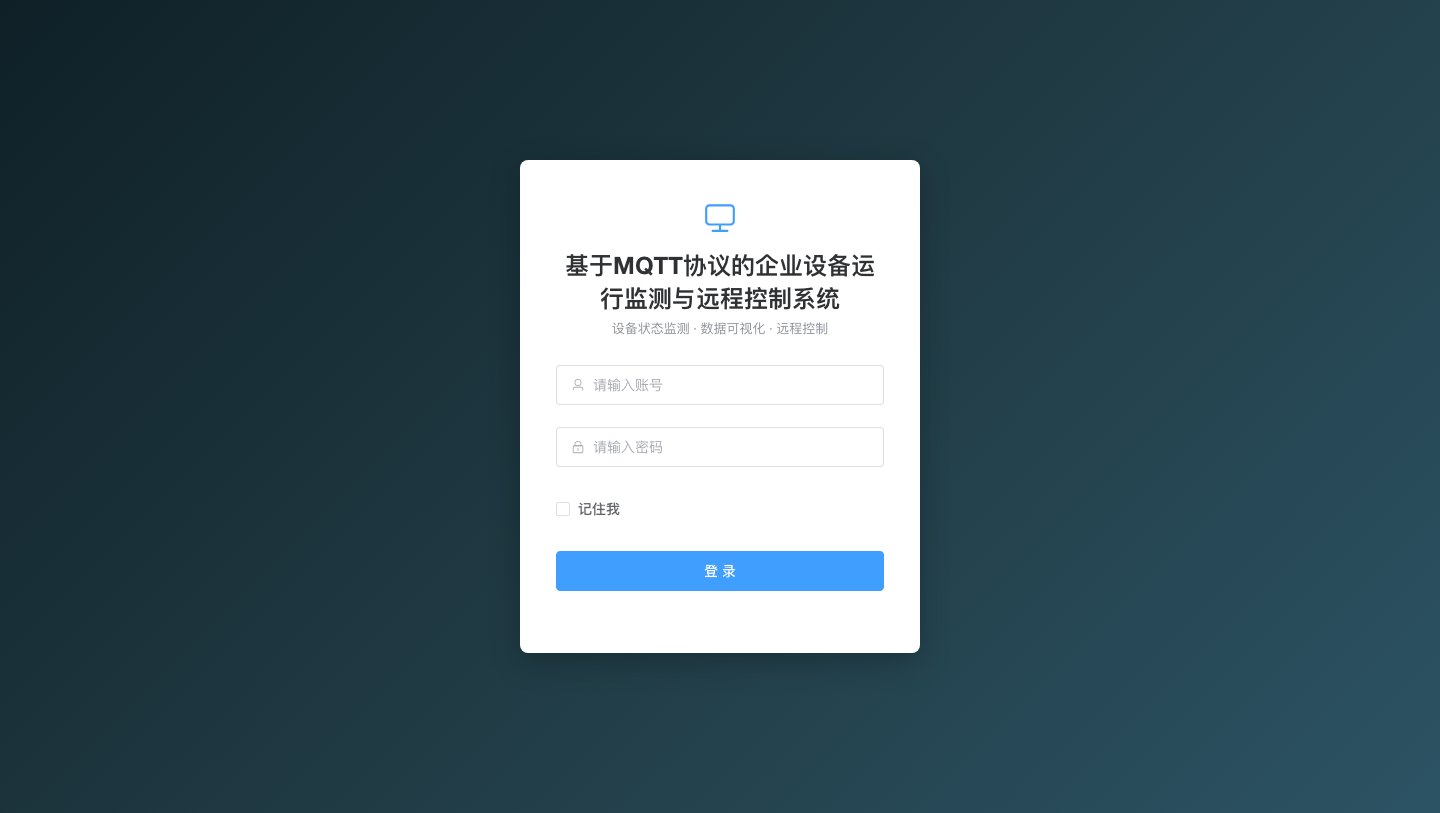
\includegraphics[width=\linewidth]{figures/login.png}
        \captionof{figure}{系统登录界面（输入 admin/123456 成功进入系统）}
        \label{fig:shot_login}
    \end{minipage}\hfill
    \begin{minipage}[t]{0.48\textwidth}
        \centering
        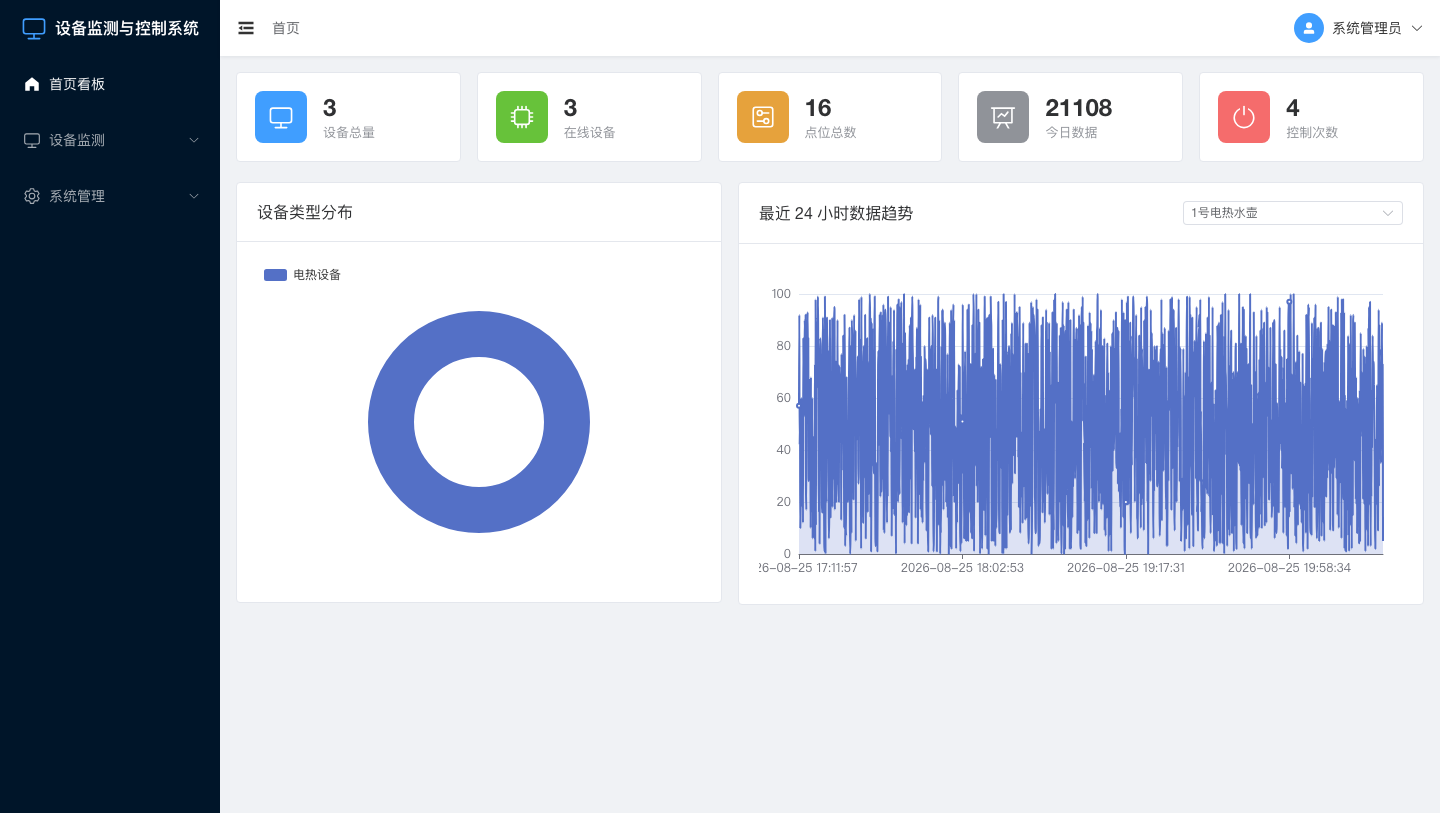
\includegraphics[width=\linewidth]{figures/dashboard.png}
        \captionof{figure}{首页统计看板（汇总卡片、设备类型分布与 24h 趋势图）}
        \label{fig:shot_dashboard}
    \end{minipage}

    \vspace{0.8em}

    \begin{minipage}[t]{0.48\textwidth}
        \centering
        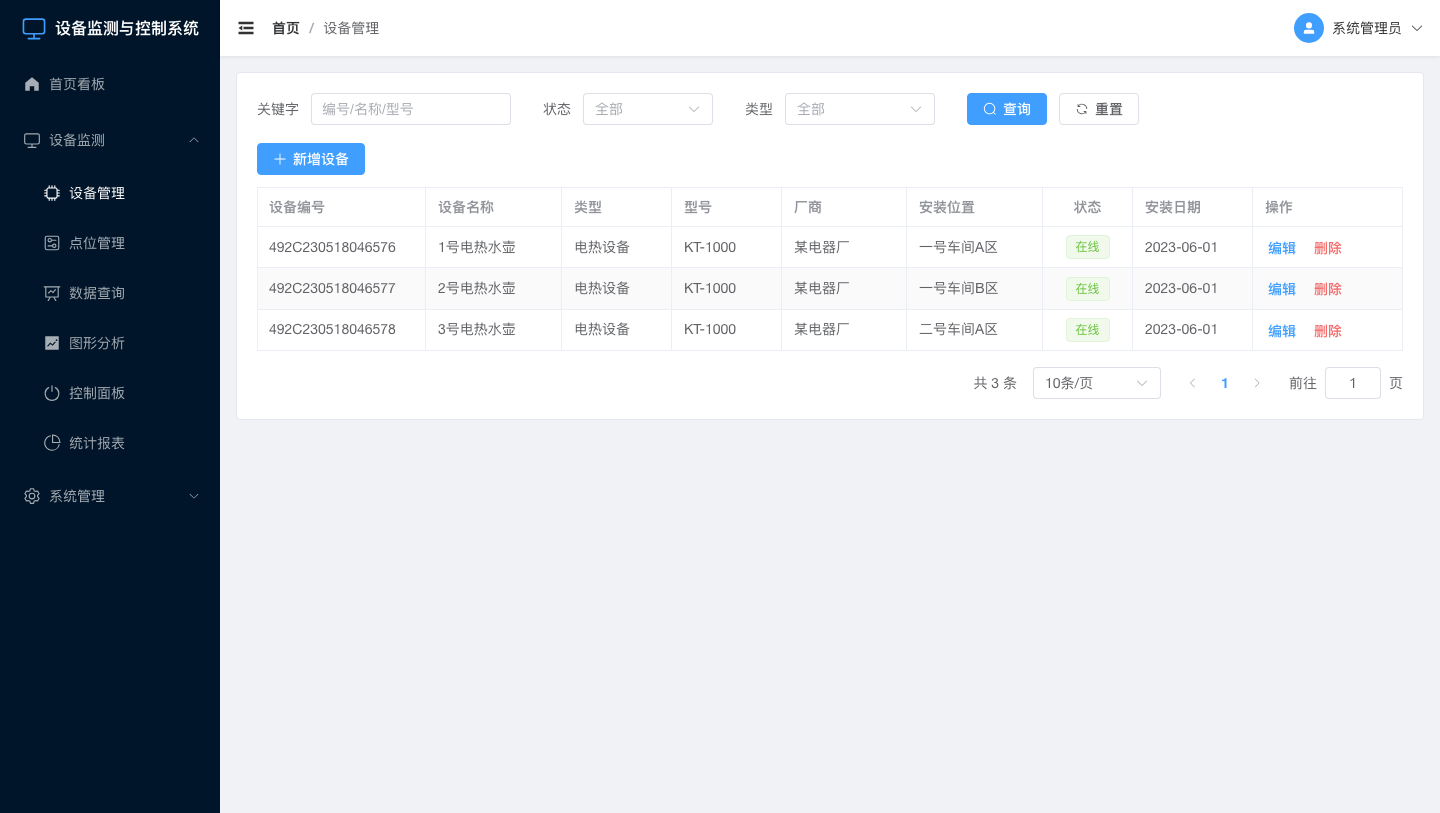
\includegraphics[width=\linewidth]{figures/device.png}
        \captionof{figure}{设备管理界面（设备台账列表与查询）}
        \label{fig:shot_device}
    \end{minipage}\hfill
    \begin{minipage}[t]{0.48\textwidth}
        \centering
        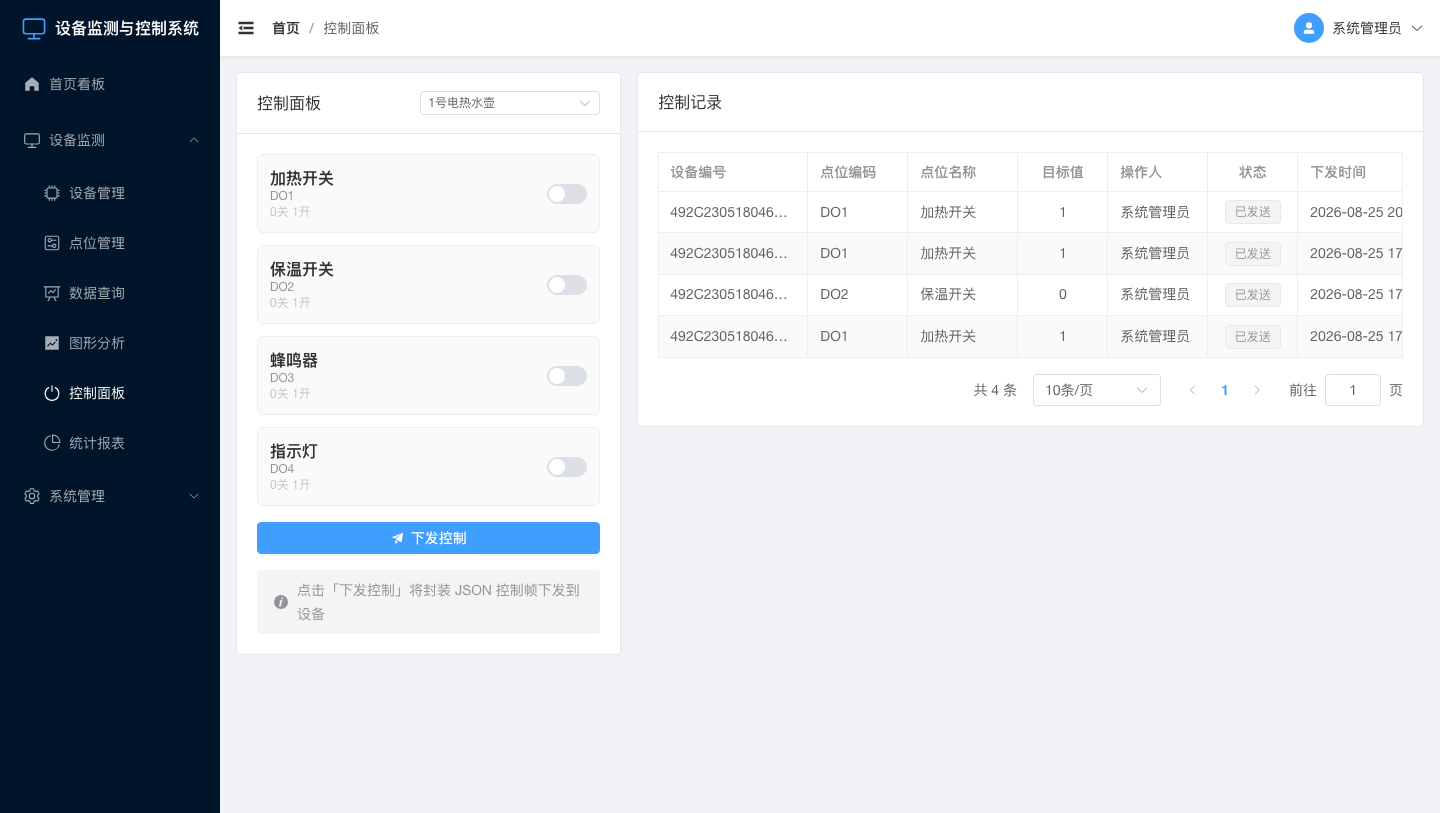
\includegraphics[width=\linewidth]{figures/control.png}
        \captionof{figure}{远程控制面板（控制点 DO1$\sim$DO4 开关）}
        \label{fig:shot_control}
    \end{minipage}

    \vspace{0.8em}

    \begin{minipage}[t]{0.48\textwidth}
        \centering
        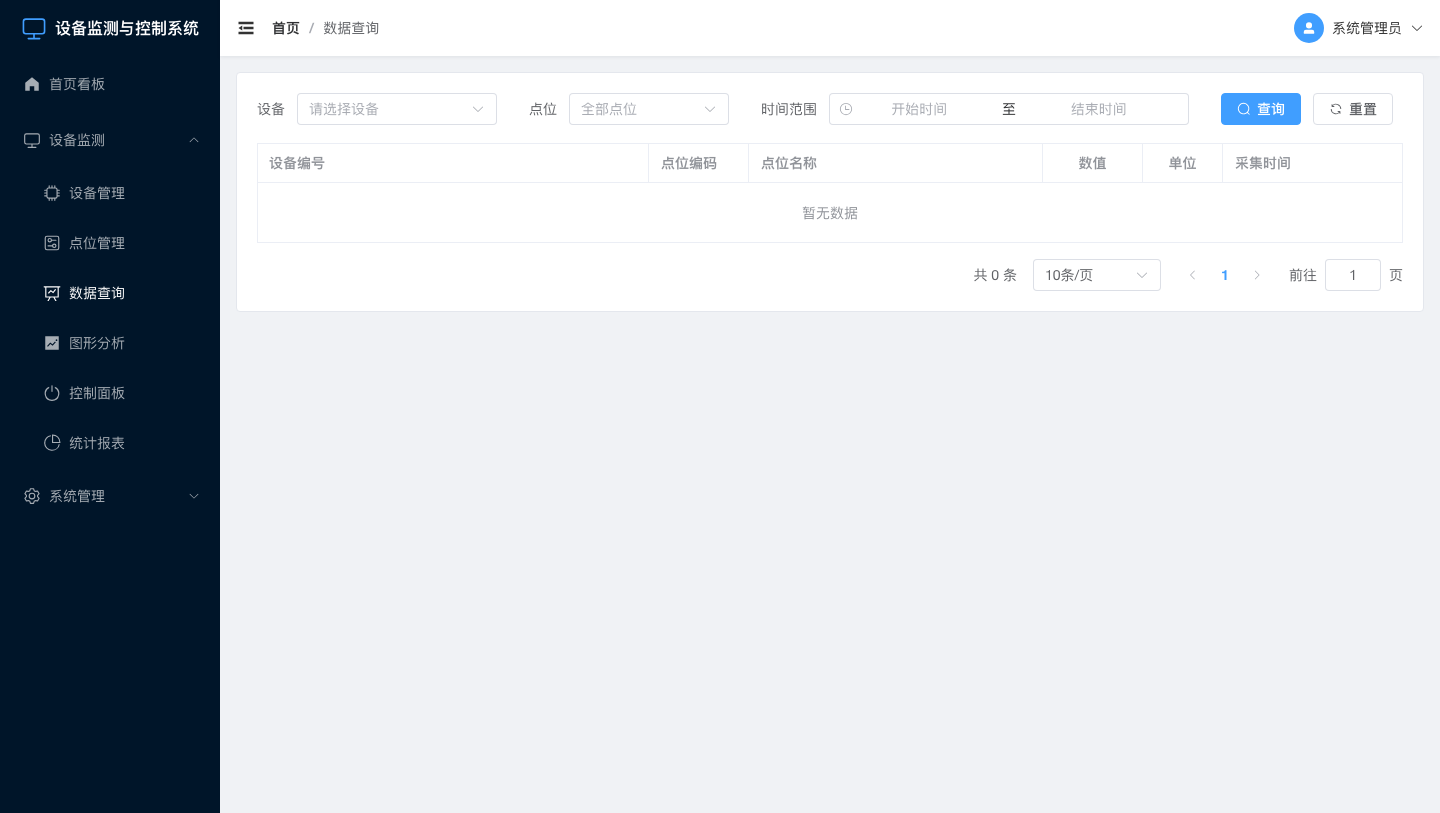
\includegraphics[width=\linewidth]{figures/data.png}
        \captionof{figure}{数据查询界面（按设备、点位与时间范围筛选）}
        \label{fig:shot_data}
    \end{minipage}\hfill
    \begin{minipage}[t]{0.48\textwidth}
        \centering
        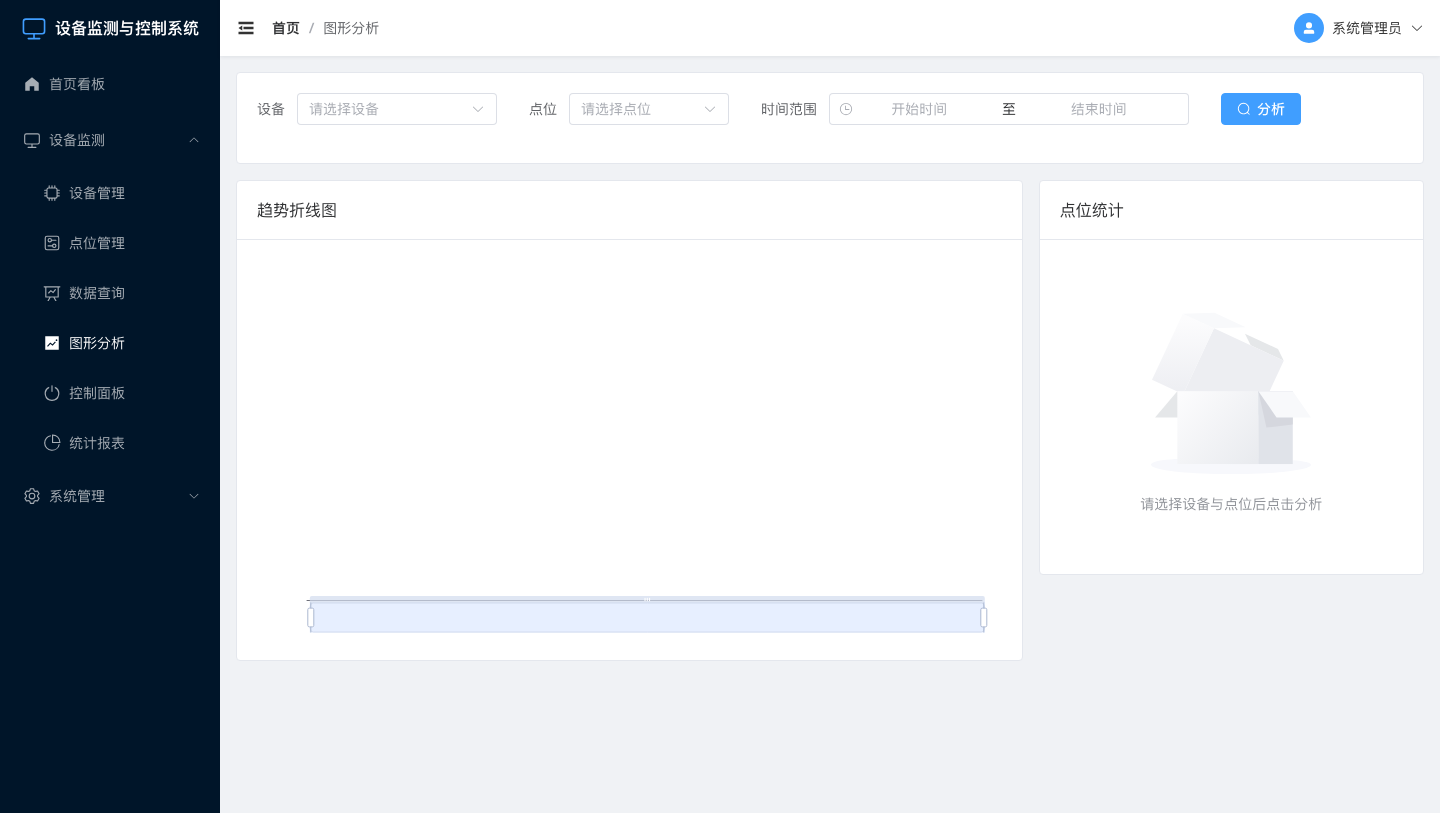
\includegraphics[width=\linewidth]{figures/chart.png}
        \captionof{figure}{图形分析界面（按设备与点位生成趋势图）}
        \label{fig:shot_chart}
    \end{minipage}
\end{center}

\FloatBarrier

%%==================== 6 结论与心得 ====================%%
\section{结论与心得}

\subsection{优点}

\begin{itemize}
    \item \textbf{架构清晰}：采用前后端分离的分层架构，各层职责明确、耦合度低，易于维护与扩展；
    \item \textbf{功能完整}：覆盖设备管理、数据采集、远程控制、报表分析、权限管理全流程，满足课程设计任务要求；
    \item \textbf{技术先进}：采用工业物联网主流 MQTT 协议与主流 Java Web 技术栈，贴近实际工程应用；
    \item \textbf{安全可靠}：密码加密存储、JWT 无状态认证、RBAC 权限控制细化到按钮级；
    \item \textbf{规范完善}：按软件工程流程完成了需求分析、数据库设计、系统设计与测试，文档齐全。
\end{itemize}

\subsection{不足}

\begin{itemize}
    \item 系统暂未实现设备异常告警与阈值报警，对异常状态的主动提示能力不足；
    \item 图形分析以折线图与饼图为主，可视化形式还可进一步丰富（如大屏驾驶舱）；
    \item 前端页面响应式适配与移动端支持有待完善；
    \item 控制下发结果的闭环确认（设备执行状态回写）可进一步细化。
\end{itemize}

\subsection{收获与体会}

通过本次课程设计，我完整经历了一个软件系统从需求分析、方案设计、编码实现到测试交付的全过程，加深了对软件工程方法与数据库设计的理解；掌握了 MQTT 协议在物联网场景下的采集与下发机制，理解了基于 JWT 与 RBAC 的权限控制原理；同时在前后端分离、分层架构方面积累了实践经验。这些能力的提升为今后从事软件开发工作打下了坚实基础。


\end{document}
